\chapter{Similarità dei Dati e Introduzione all'Analisi dei Cluster}
\label{ch:similarity-clustering}

% ============================================================
%  PARTE I – SIMILARITÀ E DISTANZA
% ============================================================

\section{Prossimità: Similarità e Dissimilarità}
\label{sec:proximity}

Ogni tecnica di Data Mining che coinvolge il confronto tra oggetti — dalla classificazione al clustering, dal recupero di informazioni alla rilevazione di anomalie — si basa su un concetto fondamentale: la \textbf{prossimità} (\textit{proximity}), termine ombrello che racchiude sia la \textit{similarità} sia la \textit{dissimilarità}.

\begin{definition}[Similarità]
La \textbf{similarità} (\textit{similarity}) è una misura numerica di quanto due oggetti dati si somiglino. Assume valore più alto quanto più gli oggetti sono simili e ricade tipicamente nell'intervallo $[0, 1]$.
\end{definition}

\begin{definition}[Dissimilarità]
La \textbf{dissimilarità} (\textit{dissimilarity}) è una misura numerica di quanto due oggetti dati differiscano tra loro. Assume valore minimo (spesso $0$) quando gli oggetti sono identici; il limite superiore varia a seconda della misura scelta.
\end{definition}

La relazione tra le due è intuitiva: a bassa dissimilarità corrisponde alta similarità e viceversa. In molti contesti pratici si utilizza una trasformazione semplice come $s = 1 - d$ oppure $s = e^{-d}$ per convertire distanza in similarità.

\subsection{Similarità e Dissimilarità per un Singolo Attributo}

Prima di affrontare il caso multidimensionale, è utile esaminare come definire la prossimità per un singolo attributo in funzione del suo tipo. La seguente tabella riassume le scelte più comuni:

\begin{table}[htbp]
\centering
\small
\begin{tabularx}{\textwidth}{>{\bfseries\raggedright\arraybackslash}p{4.2cm} >{\raggedright\arraybackslash}X >{\raggedright\arraybackslash}X}
\toprule
Tipo di Attributo & Dissimilarità & Similarità \\
\midrule
Nominale & $d = 0$ se $p = q$; \quad $d = 1$ altrimenti & $s = 1$ se $p = q$; \quad $s = 0$ altrimenti \\
\addlinespace[6pt]
Ordinale & $d = \dfrac{|p - q|}{n - 1}$ \newline {\scriptsize(valori mappati in $0, \ldots, n-1$)} & $s = 1 - d$ \\
\addlinespace[6pt]
Intervallo / Rapporto & $d = |p - q|$ & $s = -d$, \quad $s = \dfrac{1}{1+d}$, \newline oppure $s = e^{-\alpha d}$ \\
\bottomrule
\end{tabularx}
\caption{Misure di prossimità per un singolo attributo in funzione del tipo di dato.}
\label{tab:proximity-one-attr}
\end{table}

% ============================================================
\section{Distanza Euclidea e Proprietà delle Metriche}
\label{sec:euclidean}

Quando gli oggetti dati sono punti nello spazio $\mathbb{R}^n$, la misura di distanza più immediata è la \textbf{distanza euclidea}.

\begin{definition}[Distanza Euclidea]
Dati due punti $\mathbf{x} = (x_1, \ldots, x_n)$ e $\mathbf{y} = (y_1, \ldots, y_n)$ in $\mathbb{R}^n$, la \textbf{distanza euclidea} (norma $L_2$) è:
\begin{equation}
  d(\mathbf{x}, \mathbf{y}) = \sqrt{\sum_{k=1}^{n} (x_k - y_k)^2}
  \label{eq:euclidean}
\end{equation}
\end{definition}

\begin{noteblock}{Standardizzazione necessaria}
Se le scale degli attributi differiscono (ad esempio, un attributo varia in $[0,1]$ e un altro in $[0{,}000, 10{,}000]$), gli attributi con range maggiore dominano il calcolo della distanza. Prima di applicare la distanza euclidea, occorre \textbf{standardizzare} i dati (ad esempio sottraendo la media e dividendo per la deviazione standard).
\end{noteblock}

\begin{example}[Matrice delle distanze euclidee]
Consideriamo quattro punti nel piano:

\begin{center}
\begin{tabularx}{0.4\textwidth}{c c c}
\toprule
Punto & $x$ & $y$ \\
\midrule
$p_1$ & 0 & 2 \\
$p_2$ & 2 & 0 \\
$p_3$ & 3 & 1 \\
$p_4$ & 5 & 1 \\
\bottomrule
\end{tabularx}
\end{center}

Le distanze euclidee calcolate sono:

\begin{center}
\begin{tabular}{c | c c c c}
\toprule
 & $p_1$ & $p_2$ & $p_3$ & $p_4$ \\
\midrule
$p_1$ & 0 & 2.828 & 3.162 & 5.099 \\
$p_2$ & 2.828 & 0 & 1.414 & 3.162 \\
$p_3$ & 3.162 & 1.414 & 0 & 2.000 \\
$p_4$ & 5.099 & 3.162 & 2.000 & 0 \\
\bottomrule
\end{tabular}
\end{center}
\end{example}

\subsection{Proprietà di una Metrica}

Una funzione di distanza $d(\mathbf{x}, \mathbf{y})$ che rispetti le seguenti tre proprietà è chiamata \textbf{metrica}:

\begin{enumerate}
  \item \textbf{Positività e definitezza:} $d(\mathbf{x}, \mathbf{y}) \geq 0$ per ogni $\mathbf{x}, \mathbf{y}$, e $d(\mathbf{x}, \mathbf{y}) = 0$ se e solo se $\mathbf{x} = \mathbf{y}$.
  \item \textbf{Simmetria:} $d(\mathbf{x}, \mathbf{y}) = d(\mathbf{y}, \mathbf{x})$ per ogni $\mathbf{x}, \mathbf{y}$.
  \item \textbf{Disuguaglianza triangolare:} $d(\mathbf{x}, \mathbf{z}) \leq d(\mathbf{x}, \mathbf{y}) + d(\mathbf{y}, \mathbf{z})$ per ogni $\mathbf{x}, \mathbf{y}, \mathbf{z}$.
\end{enumerate}

Analogamente, una funzione di similarità $s(\mathbf{x}, \mathbf{y})$ soddisfa:
\begin{enumerate}
  \item $s(\mathbf{x}, \mathbf{y}) = 1$ (o il valore massimo) se e solo se $\mathbf{x} = \mathbf{y}$.
  \item $s(\mathbf{x}, \mathbf{y}) = s(\mathbf{y}, \mathbf{x})$ per ogni $\mathbf{x}, \mathbf{y}$ (simmetria).
\end{enumerate}

% ============================================================
\section{Distanza di Minkowski: Una Famiglia di Metriche}
\label{sec:minkowski}

La distanza euclidea è un caso particolare di una famiglia più ampia, la \textbf{distanza di Minkowski}.

\begin{definition}[Distanza di Minkowski]
Dati due punti $\mathbf{x}, \mathbf{y} \in \mathbb{R}^n$ e un parametro $r \geq 1$, la \textbf{distanza di Minkowski} (norma $L_r$) è:
\begin{equation}
  d(\mathbf{x}, \mathbf{y}) = \left( \sum_{k=1}^{n} |x_k - y_k|^r \right)^{1/r}
  \label{eq:minkowski}
\end{equation}
\end{definition}

Il parametro $r$ controlla la ``forma'' della sfera unitaria associata alla norma:

\begin{figure}[htbp]
\centering
\resizebox{0.92\linewidth}{!}{%
\begin{tikzpicture}[
  box/.style={rectangle, rounded corners=5pt, draw=blue!60!black, fill=blue!7, thick,
              minimum width=3.6cm, minimum height=2.2cm, align=center, font=\small},
  lbl/.style={font=\bfseries\small, text=blue!80!black},
  arr/.style={-Stealth, thick, gray!70}
]
  \node[box] (l1) at (0, 0) {
    $r = 1$ \\[4pt]
    \textbf{Norma $L_1$} \\[2pt]
    \scriptsize Manhattan, Taxicab \\
    \scriptsize City-block, Hamming
  };
  \node[box, draw=green!60!black, fill=green!7] (l2) at (5.5, 0) {
    $r = 2$ \\[4pt]
    \textbf{Norma $L_2$} \\[2pt]
    \scriptsize Distanza Euclidea \\
    \scriptsize (caso standard)
  };
  \node[box, draw=orange!70!black, fill=orange!8] (linf) at (11, 0) {
    $r \to \infty$ \\[4pt]
    \textbf{Norma $L_\infty$} \\[2pt]
    \scriptsize Supremum / Chebyshev \\
    \scriptsize $\max_k |x_k - y_k|$
  };
  \draw[arr] (l1.east) -- (l2.west) node[midway, above, font=\scriptsize] {più regolare};
  \draw[arr] (l2.east) -- (linf.west) node[midway, above, font=\scriptsize] {$r$ crescente};
  % Formula labels
  \node[font=\scriptsize, below=0.25cm of l1] {$\sum_k |x_k - y_k|$};
  \node[font=\scriptsize, below=0.25cm of l2] {$\sqrt{\sum_k (x_k-y_k)^2}$};
  \node[font=\scriptsize, below=0.25cm of linf] {$\max_k |x_k - y_k|$};
\end{tikzpicture}%
}
\caption{La famiglia delle norme di Minkowski al variare del parametro $r$.}
\label{fig:minkowski-family}
\end{figure}

\begin{example}[Confronto tra norme $L_1$, $L_2$, $L_\infty$]
Con gli stessi quattro punti dell'esempio precedente:

\begin{center}
\small
\begin{tabular}{c | c c c c}
\toprule
$L_1$ & $p_1$ & $p_2$ & $p_3$ & $p_4$ \\
\midrule
$p_1$ & 0 & 4 & 4 & 6 \\
$p_2$ & 4 & 0 & 2 & 4 \\
$p_3$ & 4 & 2 & 0 & 2 \\
$p_4$ & 6 & 4 & 2 & 0 \\
\bottomrule
\end{tabular}
\hspace{1cm}
\begin{tabular}{c | c c c c}
\toprule
$L_\infty$ & $p_1$ & $p_2$ & $p_3$ & $p_4$ \\
\midrule
$p_1$ & 0 & 2 & 3 & 5 \\
$p_2$ & 2 & 0 & 1 & 3 \\
$p_3$ & 3 & 1 & 0 & 2 \\
$p_4$ & 5 & 3 & 2 & 0 \\
\bottomrule
\end{tabular}
\end{center}

In $L_1$ la distanza tra $p_1$ e $p_2$ è $|0-2|+|2-0|=4$; in $L_\infty$ è $\max(|0-2|, |2-0|)=2$.
\end{example}

La norma $L_1$ è particolarmente utile nei dati ad alta dimensionalità e sparsi, e la \textbf{distanza di Hamming} — il numero di bit diversi tra due vettori binari — ne è un caso speciale.

% ============================================================
\section{Similarità tra Dati Binari}
\label{sec:binary-similarity}

Quando gli attributi sono \textbf{binari} (presenti/assenti, vero/falso), la nozione di distanza euclidea perde di significato semantico. Si preferisce invece ragionare in termini di \textit{corrispondenze}.

Dati due oggetti $p$ e $q$ con attributi binari, definiamo la seguente \textbf{tabella di contingenza}:

\begin{center}
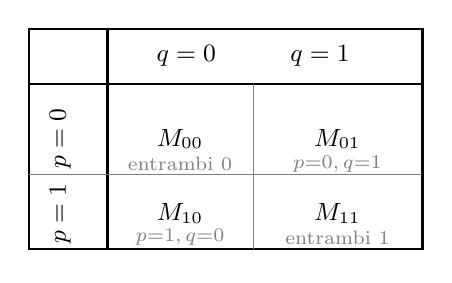
\begin{tikzpicture}[font=\small]
  % outer border
  \draw[thick] (-0.5, -1.8) rectangle (4.5, 1.0);
  % header row
  \node at (1.5, 0.65) {\textbf{$q=0$}};
  \node at (3.2, 0.65) {\textbf{$q=1$}};
  \node at (-0.1, -0.4) [rotate=90] {\textbf{$p=0$}};
  \node at (-0.1, -1.35) [rotate=90] {\textbf{$p=1$}};
  % dividers
  \draw[thick] (-0.5, 0.3) -- (4.5, 0.3);
  \draw[thick] (0.5, -1.8) -- (0.5, 1.0);
  \draw[gray] (2.35, -1.8) -- (2.35, 0.3);
  \draw[gray] (-0.5, -0.85) -- (4.5, -0.85);
  % cells
  \node at (1.42, -0.4)  {$M_{00}$};
  \node at (3.42, -0.4)  {$M_{01}$};
  \node at (1.42, -1.35) {$M_{10}$};
  \node at (3.42, -1.35) {$M_{11}$};
  % labels
  \node[font=\scriptsize, text=gray] at (1.42, -0.72) {entrambi 0};
  \node[font=\scriptsize, text=gray] at (3.42, -0.72) {$p{=}0, q{=}1$};
  \node[font=\scriptsize, text=gray] at (1.42, -1.65) {$p{=}1, q{=}0$};
  \node[font=\scriptsize, text=gray] at (3.42, -1.65) {entrambi 1};
\end{tikzpicture}
\end{center}

\begin{definition}[Simple Matching Coefficient — SMC]
\begin{equation}
  \mathrm{SMC}(p, q) = \frac{M_{11} + M_{00}}{M_{01} + M_{10} + M_{11} + M_{00}}
  \label{eq:smc}
\end{equation}
Conta sia le corrispondenze $1\text{-}1$ che le corrispondenze $0\text{-}0$.
\end{definition}

\begin{definition}[Coefficiente di Jaccard]
\begin{equation}
  J(p, q) = \frac{M_{11}}{M_{01} + M_{10} + M_{11}}
  \label{eq:jaccard}
\end{equation}
Ignora le corrispondenze $0\text{-}0$: è adatto quando l'assenza di un attributo non è informativa (es.\ insiemi di acquisti, tag, malattie rare).
\end{definition}

\begin{example}[SMC vs.\ Jaccard]
Siano:
\[
  p = [1, 0, 0, 0, 0, 0, 0, 0, 0, 0], \quad q = [0, 0, 0, 0, 0, 0, 1, 0, 0, 1]
\]
\begin{itemize}
  \item $M_{11} = 0$ (nessuna corrispondenza $1\text{-}1$)
  \item $M_{10} = 1$ (solo $p_1=1$ con $q_1=0$)
  \item $M_{01} = 2$ ($q_7=1$ e $q_{10}=1$ mentre $p=0$)
  \item $M_{00} = 7$ (entrambi 0 per le restanti posizioni)
\end{itemize}
\[
  \mathrm{SMC} = \frac{0+7}{2+1+0+7} = 0.7, \qquad J = \frac{0}{2+1+0} = 0
\]
SMC è alta perché conta i 7 zeri in comune; Jaccard è 0 perché non vi è nessuna co-occorrenza di 1. Per dati di tipo \textit{market basket} (dove l'assenza di un prodotto non è informativa), Jaccard è la scelta corretta.
\end{example}

% ============================================================
\section{Similarità del Coseno}
\label{sec:cosine}

Nei dati documentali (vettori di frequenze di parole, \textit{TF-IDF}), i vettori tendono ad essere ad alta dimensionalità e sparsi. La distanza euclidea è sensibile alla lunghezza del documento; la \textbf{similarità del coseno} normalizza per la norma e misura solo l'angolo tra i vettori.

\begin{definition}[Similarità del Coseno]
Dati due vettori $\mathbf{d}_1, \mathbf{d}_2 \in \mathbb{R}^n$:
\begin{equation}
  \cos(\mathbf{d}_1, \mathbf{d}_2) = \frac{\mathbf{d}_1 \cdot \mathbf{d}_2}{\|\mathbf{d}_1\| \, \|\mathbf{d}_2\|}
  \label{eq:cosine}
\end{equation}
dove $\mathbf{d}_1 \cdot \mathbf{d}_2 = \sum_{k} d_{1k} \cdot d_{2k}$ è il prodotto scalare e $\|\mathbf{d}\| = \sqrt{\sum_k d_k^2}$ è la norma euclidea.
\end{definition}

Il valore ricade in $[-1, 1]$; per vettori non negativi (come le frequenze di parole) il range è $[0, 1]$: $1$ indica direzioni identiche, $0$ indica vettori ortogonali.

\begin{example}[Cosine Similarity su documenti]
\begin{align*}
  \mathbf{d}_1 &= [3, 2, 0, 5, 0, 0, 0, 2, 0, 0] \\
  \mathbf{d}_2 &= [1, 0, 0, 0, 0, 0, 0, 1, 0, 2]
\end{align*}
\[
  \mathbf{d}_1 \cdot \mathbf{d}_2 = 3{\cdot}1 + 2{\cdot}0 + 5{\cdot}0 + 2{\cdot}1 = 5
\]
\[
  \|\mathbf{d}_1\| = \sqrt{9+4+25+4} = \sqrt{42} \approx 6.481, \quad
  \|\mathbf{d}_2\| = \sqrt{1+1+4} = \sqrt{6} \approx 2.449
\]
\[
  \cos(\mathbf{d}_1, \mathbf{d}_2) = \frac{5}{6.481 \times 2.449} \approx 0.315
\]
I documenti condividono circa il 31.5\% di ``direzione'', nonostante la diversa lunghezza.
\end{example}

\subsection{Similarità Pesata}

In molti casi non tutti gli attributi contribuiscono equalmente alla similarità. Si può definire una \textbf{similarità pesata} introducendo pesi non negativi $w_k$ con $\sum_k w_k = 1$:
\begin{equation}
  s_w(\mathbf{x}, \mathbf{y}) = \frac{\sum_{k=1}^{n} w_k \cdot d_k \cdot s_k(x_k, y_k)}{\sum_{k=1}^{n} w_k \cdot d_k}
\end{equation}
dove $s_k$ è la similarità per il $k$-esimo attributo e $d_k$ è un fattore di normalizzazione.

% ============================================================
\section{Correlazione}
\label{sec:correlation}

La \textbf{correlazione di Pearson} misura la relazione \textit{lineare} tra due variabili (o tra due oggetti visti come vettori di attributi). Si calcola standardizzando i vettori e calcolando il loro prodotto scalare:
\begin{equation}
  \mathrm{corr}(p, q) = \frac{\sum_{k=1}^{n}(p_k - \bar{p})(q_k - \bar{q})}{(n-1)\,\sigma_p\,\sigma_q}
  \label{eq:pearson}
\end{equation}
dove $\bar{p}, \bar{q}$ sono le medie e $\sigma_p, \sigma_q$ le deviazioni standard. Il risultato ricade in $[-1, 1]$:
\begin{itemize}
  \item $+1$: correlazione positiva perfetta (i valori crescono insieme);
  \item $0$: nessuna correlazione lineare;
  \item $-1$: correlazione negativa perfetta (uno cresce mentre l'altro decresce).
\end{itemize}

% ============================================================
\section{Misure Basate sull'Informazione: Entropia e Mutua Informazione}
\label{sec:entropy}

Le misure basate sulla \textbf{teoria dell'informazione} consentono di quantificare la prossimità tra variabili categoriali o continue in modo non lineare, andando oltre il semplice confronto valore-per-valore.

\subsection{Entropia}

L'informazione contenuta in un evento è inversamente proporzionale alla sua probabilità: un evento certissimo non trasmette informazione, uno raro ne trasmette molta.

\begin{definition}[Entropia di Shannon]
Per una variabile discreta $X$ con $n$ possibili valori $x_1, \ldots, x_n$ e probabilità $p_1, \ldots, p_n$:
\begin{equation}
  H(X) = -\sum_{i=1}^{n} p_i \log_2 p_i
  \label{eq:entropy}
\end{equation}
L'entropia è misurata in \textbf{bit} e ricade in $[0, \log_2 n]$.
\end{definition}

Casi limite:
\begin{itemize}
  \item Se una probabilità è 1 (evento certo), $H = 0$ — massima certezza, zero informazione.
  \item Se tutti i valori sono equiprobabili ($p_i = 1/n$), $H = \log_2 n$ — massima incertezza.
\end{itemize}

\begin{example}[Moneta equa vs.\ truccata]
Per una moneta con probabilità $p$ di testa e $q = 1-p$ di croce:
\[
  H = -p \log_2 p - q \log_2 q
\]
Con $p=0.5$ (moneta equa): $H = 1$ bit. Con $p=1$ o $p=0$ (moneta truccata): $H = 0$ bit.
\end{example}

\subsection{Mutua Informazione}

La \textbf{mutua informazione} (\textit{Mutual Information}, MI) quantifica quanta informazione una variabile $X$ fornisce su un'altra variabile $Y$:

\begin{definition}[Mutua Informazione]
\begin{equation}
  I(X; Y) = H(X) + H(Y) - H(X, Y)
  \label{eq:mutual-info}
\end{equation}
dove $H(X,Y) = -\sum_i \sum_j p_{ij} \log_2 p_{ij}$ è l'entropia congiunta e $p_{ij} = P(X = x_i, Y = y_j)$.
\end{definition}

$I(X;Y) = 0$ se $X$ e $Y$ sono indipendenti. Il valore massimo per variabili discrete è $\log_2(\min(n_X, n_Y))$. A differenza della correlazione di Pearson, la MI cattura anche dipendenze \textit{non lineari}.

\begin{example}[Mutua Informazione: Studenti e Voti]
Consideriamo le variabili \textit{Status dello Studente} (Undergraduate/Graduate) e \textit{Voto} (A/B/C) su 100 studenti:

\begin{center}
\small
\begin{tabularx}{0.85\linewidth}{l r r r}
\toprule
& \multicolumn{2}{c}{\textbf{Status}} & \\
\textbf{Voto} & Undergrad & Grad & Totale \\
\midrule
A & 5 & 30 & 35 \\
B & 30 & 20 & 50 \\
C & 10 & 5  & 15 \\
\midrule
Totale & 45 & 55 & 100 \\
\bottomrule
\end{tabularx}
\end{center}

$H(\text{Status}) = -(0.45\log_2 0.45 + 0.55\log_2 0.55) \approx 0.993$ bit

$H(\text{Voto}) = -(0.35\log_2 0.35 + 0.50\log_2 0.50 + 0.15\log_2 0.15) \approx 1.441$ bit

$H(\text{Status}, \text{Voto}) \approx 2.271$ bit

\[
  I(\text{Status}; \text{Voto}) = 0.993 + 1.441 - 2.271 \approx \mathbf{0.163} \text{ bit}
\]
La MI positiva indica che conoscere lo status fornisce (poca) informazione sul voto e viceversa.
\end{example}

% ============================================================
%  PARTE II – ANALISI DEI CLUSTER
% ============================================================

\section{Che cos'è l'Analisi dei Cluster?}
\label{sec:cluster-analysis}

\begin{definition}[Cluster Analysis]
La \textbf{cluster analysis} (o \textbf{clustering}) è il processo di raggruppamento di un insieme di oggetti in \textbf{cluster}, ovvero gruppi tali che:
\begin{itemize}
  \item gli oggetti \textit{all'interno} dello stesso cluster siano il più possibile simili tra loro (\textit{alta coesione intra-cluster});
  \item gli oggetti di cluster \textit{diversi} siano il più possibile dissimili (\textit{alta separazione inter-cluster}).
\end{itemize}
\end{definition}

\begin{figure}[htbp]
\centering
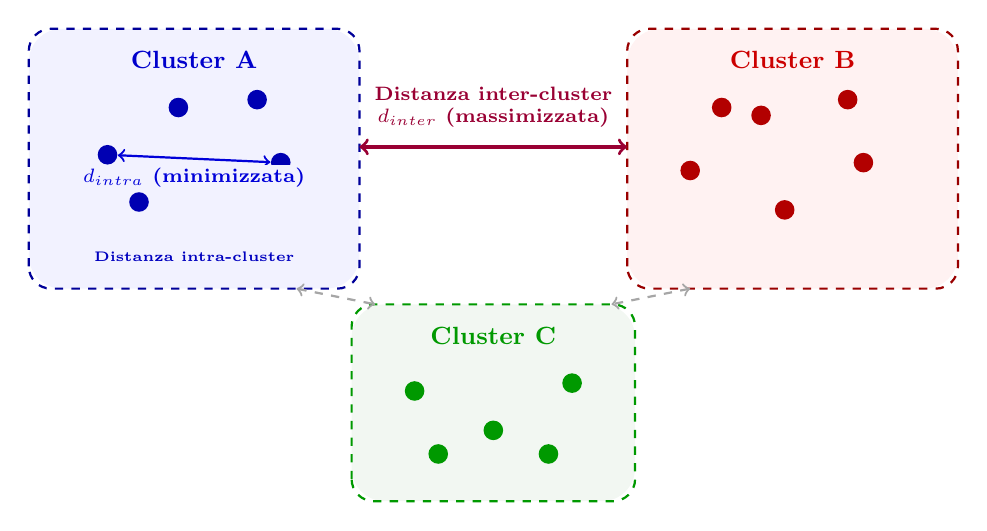
\begin{tikzpicture}[
  dotA/.style={circle, fill=blue!70!black, inner sep=2.5pt},
  dotB/.style={circle, fill=red!70!black, inner sep=2.5pt},
  dotC/.style={circle, fill=green!60!black, inner sep=2.5pt},
  clusterbox/.style={dashed, thick, rounded corners=8pt}
]
  % Cluster A (sinistra) - larghezza 4.2cm
  \fill[blue!5, rounded corners=12pt] (0.0, 0.6) rectangle (4.2, 3.9);
  \draw[blue!60!black, clusterbox] (0.0, 0.6) rectangle (4.2, 3.9);
  \node[font=\small\bfseries, text=blue!80!black] at (2.1, 3.5) {Cluster A};
  
  \node[dotA] (a1) at (1.0, 2.3) {};
  \node[dotA] (a2) at (1.9, 2.9) {};
  \node[dotA] (a3) at (3.2, 2.2) {};
  \node[dotA] at (1.4, 1.7) {};
  \node[dotA] at (2.9, 3.0) {};
  
  % Distanza intra-cluster interna a Cluster A
  \draw[<->, thick, blue!85!black] (a1) -- (a3)
    node[midway, below=2pt, font=\scriptsize\bfseries, fill=blue!5, inner sep=1pt] {$d_{\text{intra}}$ (minimizzata)};
  \node[font=\tiny\bfseries, text=blue!75!black, align=center] at (2.1, 1.0) {Distanza intra-cluster};

  % Cluster B (destra) - larghezza 4.2cm
  \fill[red!5, rounded corners=12pt] (7.6, 0.6) rectangle (11.8, 3.9);
  \draw[red!60!black, clusterbox] (7.6, 0.6) rectangle (11.8, 3.9);
  \node[font=\small\bfseries, text=red!80!black] at (9.7, 3.5) {Cluster B};
  
  \node[dotB] at (8.4, 2.1) {};
  \node[dotB] at (9.3, 2.8) {};
  \node[dotB] at (10.6, 2.2) {};
  \node[dotB] at (8.8, 2.9) {};
  \node[dotB] at (10.4, 3.0) {};
  \node[dotB] at (9.6, 1.6) {};

  % Distanza inter-cluster tra Cluster A e Cluster B
  \draw[<->, very thick, purple!80!black] (4.2, 2.4) -- (7.6, 2.4)
    node[midway, above=3pt, font=\scriptsize\bfseries, align=center] {Distanza inter-cluster\\$d_{\text{inter}}$ (massimizzata)};

  % Cluster C (in basso, centrato tra A e B)
  \fill[green!40!black!5, rounded corners=12pt] (4.1, -2.1) rectangle (7.7, 0.4);
  \draw[green!60!black, clusterbox] (4.1, -2.1) rectangle (7.7, 0.4);
  \node[font=\small\bfseries, text=green!60!black] at (5.9, 0.0) {Cluster C};

  \node[dotC] at (4.9, -0.7) {};
  \node[dotC] at (5.9, -1.2) {};
  \node[dotC] at (6.9, -0.6) {};
  \node[dotC] at (5.2, -1.5) {};
  \node[dotC] at (6.6, -1.5) {};

  % Connessioni tratteggiate verso Cluster C
  \draw[<->, dashed, thick, gray!70] (3.4, 0.6) -- (4.4, 0.4);
  \draw[<->, dashed, thick, gray!70] (8.4, 0.6) -- (7.4, 0.4);
\end{tikzpicture}
\caption{Obiettivo fondamentale del clustering: massimizzare le distanze inter-cluster (separazione) e minimizzare le distanze intra-cluster (coesione).}
\label{fig:clustering-objective}
\end{figure}

Il clustering è un'attività di \textbf{apprendimento non supervisionato}: a differenza della classificazione, non si dispone di etichette predefinite. L'algoritmo deve scoprire autonomamente la struttura latente nei dati.

\subsection{Applicazioni del Clustering}

Il clustering trova applicazione in una vasta gamma di domini:

\begin{itemize}
  \item \textbf{Comprensione:} raggruppare documenti per argomento (information retrieval), raggruppare geni con funzionalità simile (bioinformatica), raggruppare azioni con andamento correlato (finanza).
  \item \textbf{Riepilogo e compressione:} ridurre un dataset di grandi dimensioni sostituendo ogni cluster con un rappresentante (centroide o medoide), utile per la visualizzazione e per la pre-elaborazione di altri algoritmi.
  \item \textbf{Rilevamento di anomalie:} oggetti che non appartengono a nessun cluster (o a cluster molto piccoli) sono potenziali anomalie.
  \item \textbf{Clustering spaziale:} scoprire zone geografiche con caratteristiche ambientali simili (es.\ precipitazioni in Australia).
\end{itemize}

\subsection{Cosa NON è il Clustering}

È importante non confondere il clustering con altri processi superficialmente simili:

\begin{itemize}
  \item \textbf{Segmentazione semplice:} dividere gli studenti in gruppi alfabetici per cognome è una partizione, non un clustering — i gruppi sono definiti da una regola esterna, non dalla similarità dei dati.
  \item \textbf{Risultati di una query:} recuperare tutti i documenti che contengono la parola ``machine learning'' produce un insieme, non un clustering — la specifica del gruppo è esterna.
  \item \textbf{Classificazione supervisionata:} le etichette di classe sono fornite a priori; il clustering le deve scoprire.
  \item \textbf{Association Analysis:} trova relazioni locali tra item (es.\ regole di associazione); il clustering cerca strutture globali di raggruppamento.
\end{itemize}

% ============================================================
\section{Ambiguità e Soggettività del Concetto di Cluster}
\label{sec:cluster-ambiguity}

\begin{alertblock}{Il clustering non ha un'unica risposta corretta}
La stessa nuvola di punti può essere validamente interpretata come 2, 4 o 6 cluster a seconda della scala di analisi, della misura di prossimità scelta e dell'algoritmo impiegato. Non esiste una risposta ``oggettivamente corretta'': il clustering è sempre relativo al modello e al contesto.
\end{alertblock}

Questo fatto impone cautela nell'interpretazione dei risultati e rende indispensabile la valutazione qualitativa e quantitativa della bontà del clustering ottenuto.

% ============================================================
\section{Tassonomia dei Clustering}
\label{sec:clustering-types}

Un \textbf{clustering} è un insieme di cluster che partizioni o organizza gli oggetti. Esistono diverse tassonomie ortogonali.

\subsection{Clustering Partizionale vs.\ Gerarchico}

\begin{figure}[htbp]
\centering
\resizebox{\linewidth}{!}{%
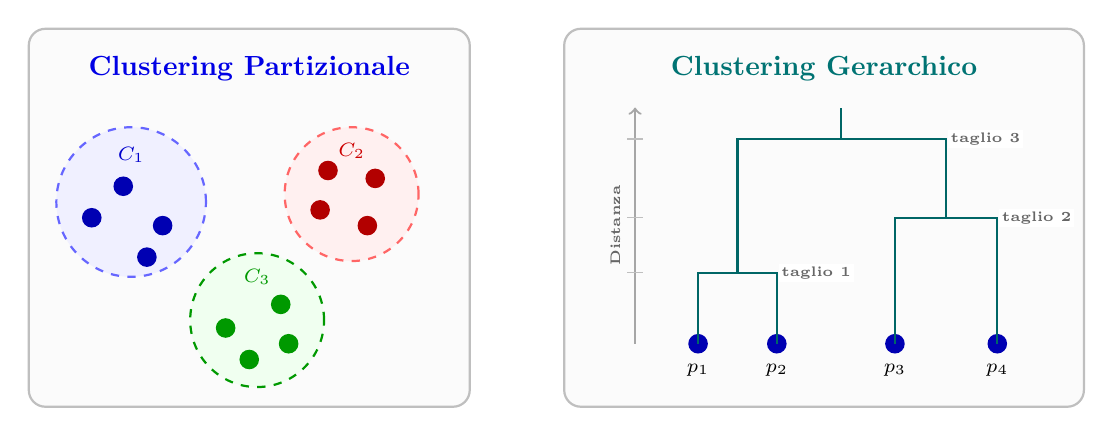
\begin{tikzpicture}[
  dot/.style={circle, fill=blue!70!black, inner sep=2.5pt},
  rdot/.style={circle, fill=red!70!black, inner sep=2.5pt},
  gdot/.style={circle, fill=green!60!black, inner sep=2.5pt},
  boxpanel/.style={draw=gray!50, thick, rounded corners=6pt, fill=gray!3}
]
  % === PANNELLO SINISTRO: Clustering Partizionale ===
  \draw[boxpanel] (-0.2, -0.2) rectangle (5.4, 4.6);
  \node[font=\bfseries\normalsize, text=blue!90!black] at (2.6, 4.1) {Clustering Partizionale};

  % Cluster 1
  \draw[blue!60, dashed, thick, fill=blue!6] (1.1, 2.4) circle(0.95);
  \node[font=\scriptsize\bfseries, text=blue!80!black] at (1.1, 3.0) {$C_1$};
  \node[dot] at (0.6, 2.2) {};
  \node[dot] at (1.0, 2.6) {};
  \node[dot] at (1.5, 2.1) {};
  \node[dot] at (1.3, 1.7) {};

  % Cluster 2
  \draw[red!60, dashed, thick, fill=red!6] (3.9, 2.5) circle(0.85);
  \node[font=\scriptsize\bfseries, text=red!80!black] at (3.9, 3.05) {$C_2$};
  \node[rdot] at (3.5, 2.3) {};
  \node[rdot] at (4.2, 2.7) {};
  \node[rdot] at (4.1, 2.1) {};
  \node[rdot] at (3.6, 2.8) {};

  % Cluster 3
  \draw[green!60!black, dashed, thick, fill=green!6] (2.7, 0.9) circle(0.85);
  \node[font=\scriptsize\bfseries, text=green!60!black] at (2.7, 1.45) {$C_3$};
  \node[gdot] at (2.3, 0.8) {};
  \node[gdot] at (3.0, 1.1) {};
  \node[gdot] at (2.6, 0.4) {};
  \node[gdot] at (3.1, 0.6) {};

  % === PANNELLO DESTRO: Clustering Gerarchico ===
  \draw[boxpanel] (6.6, -0.2) rectangle (13.2, 4.6);
  \node[font=\bfseries\normalsize, text=teal!90!black] at (9.9, 4.1) {Clustering Gerarchico};

  % Asse dei livelli / distanza
  \draw[->, thick, gray!70] (7.5, 0.6) -- (7.5, 3.6);
  \node[font=\tiny\bfseries, text=gray!80!black, rotate=90] at (7.25, 2.1) {Distanza};
  \draw[gray!50] (7.4, 1.5) -- (7.6, 1.5);
  \draw[gray!50] (7.4, 2.2) -- (7.6, 2.2);
  \draw[gray!50] (7.4, 3.2) -- (7.6, 3.2);

  % Punti foglia
  \node[dot, label={below:\scriptsize $p_1$}] (p1) at (8.3, 0.6) {};
  \node[dot, label={below:\scriptsize $p_2$}] (p2) at (9.3, 0.6) {};
  \node[dot, label={below:\scriptsize $p_3$}] (p3) at (10.8, 0.6) {};
  \node[dot, label={below:\scriptsize $p_4$}] (p4) at (12.1, 0.6) {};

  % Dendrogramma
  % Fusione 1: p1 e p2 a quota 1.5
  \draw[thick, teal!80!black] (p1.center) -- (8.3, 1.5) -- (9.3, 1.5) -- (p2.center);
  \node[font=\tiny\bfseries, fill=white, inner sep=1pt, text=gray!80!black] at (9.8, 1.5) {taglio 1};

  % Fusione 2: p3 e p4 a quota 2.2
  \draw[thick, teal!80!black] (p3.center) -- (10.8, 2.2) -- (12.1, 2.2) -- (p4.center);
  \node[font=\tiny\bfseries, fill=white, inner sep=1pt, text=gray!80!black] at (12.6, 2.2) {taglio 2};

  % Fusione 3: radice a quota 3.2
  \draw[thick, teal!80!black] (8.8, 1.5) -- (8.8, 3.2) -- (11.45, 3.2) -- (11.45, 2.2);
  \draw[thick, teal!80!black] (10.12, 3.2) -- (10.12, 3.6);
  \node[font=\tiny\bfseries, fill=white, inner sep=1pt, text=gray!80!black] at (11.95, 3.2) {taglio 3};
\end{tikzpicture}%
}
\caption{Clustering partizionale (partizioni disgiunte non sovrapposte) a confronto con il clustering gerarchico (dendrogramma annidato con livelli di aggregazione).}
\label{fig:partitional-vs-hierarchical}
\end{figure}

\begin{definition}[Clustering Partizionale]
Un \textbf{clustering partizionale} divide gli oggetti in $k$ sottoinsiemi disgiunti (cluster) tali che ogni oggetto appartiene ad esattamente un cluster.
\end{definition}

\begin{definition}[Clustering Gerarchico]
Un \textbf{clustering gerarchico} produce un insieme di cluster annidati organizzato come un albero (\textit{dendrogramma}). A ogni livello dell'albero corrisponde una diversa granularità del raggruppamento.
\end{definition}

\subsection{Altre Distinzioni}

\begin{itemize}
  \item \textbf{Esclusivo vs.\ Non-esclusivo:} nel clustering non-esclusivo (\textit{soft} o \textit{overlapping}), un punto può appartenere a più cluster simultaneamente (ad es.\ un punto di confine).
  \item \textbf{Fuzzy vs.\ Non-fuzzy:} nel clustering fuzzy, ogni punto appartiene a ogni cluster con un peso $w_{ik} \in [0,1]$ tale che $\sum_k w_{ik} = 1$. Il clustering probabilistico ha caratteristiche simili.
  \item \textbf{Parziale vs.\ Completo:} talvolta si vuole raggruppare solo un sottoinsieme dei dati (ad es.\ escludendo i rumori).
  \item \textbf{Omogeneo vs.\ Eterogeneo:} cluster di dimensioni, forme e densità molto diverse.
\end{itemize}

% ============================================================
\section{Tipologie di Cluster}
\label{sec:cluster-definitions}

Il termine ``cluster'' può avere significati molto diversi a seconda del modello adottato. Le cinque tipologie principali sono:

\subsection{Cluster Ben Separati (\textit{Well-Separated})}

\begin{definition}[Cluster Ben Separato]
Un cluster ben separato è un insieme di punti tali che ogni punto è più vicino (o simile) a ogni altro punto del suo cluster che a qualsiasi punto di un cluster diverso.
\end{definition}

Questa definizione intuitiva funziona bene quando i cluster sono effettivamente compatti e distanziati, ma fallisce in presenza di cluster elongati, di forme irregolari o di rumore.

\subsection{Cluster Basati sul Centro (\textit{Center-Based})}

\begin{definition}[Cluster Center-Based]
Un cluster center-based è un insieme di oggetti tali che ogni oggetto è più vicino (simile) al \textbf{centro} del suo cluster che al centro di qualunque altro cluster. Il centro può essere:
\begin{itemize}
  \item il \textbf{centroide}: media (vettore) di tutti i punti del cluster;
  \item il \textbf{medoide}: il punto reale del cluster più rappresentativo (minimizza la distanza media agli altri).
\end{itemize}
\end{definition}

Questa è la definizione alla base degli algoritmi \textit{K-means} e \textit{K-medoids}.

\subsection{Cluster per Contiguità (\textit{Contiguity-Based})}

\begin{definition}[Cluster Contiguo]
Un cluster contiguo (o basato sul vicinato transitivo) è un insieme di punti tale che ogni punto è più vicino ad almeno un altro punto del suo cluster che a qualsiasi punto di un altro cluster.
\end{definition}

Questo approccio produce strutture basate su grafi (ogni punto è connesso ai suoi vicini più prossimi). È sensibile al \textbf{rumore}: anche un singolo punto intermedio (``ponte'') tra due cluster distinti può unirli erroneamente.

\subsection{Cluster Basati sulla Densità (\textit{Density-Based})}

\begin{definition}[Cluster Density-Based]
Un cluster density-based è una regione densa di punti separata da regioni a bassa densità da altre regioni dense.
\end{definition}

Questa definizione consente di scoprire cluster di forma arbitraria e gestisce in modo naturale rumori e outlier (che rimangono isolati nelle regioni a bassa densità). È alla base di algoritmi come DBSCAN.

\subsection{Cluster Definiti da una Funzione Obiettivo}

Un approccio alternativo consiste nel definire una \textbf{funzione obiettivo} $f$ e cercare la partizione che la minimizza o massimizza. Il problema è in generale \textbf{NP-hard}: enumerare tutte le partizioni possibili ha costo esponenziale nel numero di punti.

\begin{itemize}
  \item Gli algoritmi \textbf{gerarchici} tipicamente ottimizzano \textit{obiettivi locali} (fusioni o divisioni greedy).
  \item Gli algoritmi \textbf{partizionali} (come K-means) tipicamente ottimizzano \textit{obiettivi globali} (es.\ somma delle distanze al centroide).
\end{itemize}

La seguente tabella confronta sinteticamente le cinque tipologie:

\begin{table}[htbp]
\centering
\small
\begin{tabularx}{\textwidth}{>{\bfseries}p{3.2cm} >{\raggedright\arraybackslash}X >{\raggedright\arraybackslash}X}
\toprule
Tipologia & Criterio di appartenenza & Algoritmi tipici \\
\midrule
Well-Separated & Più vicino a tutti i punti del proprio cluster & --- (definizione ideale) \\
\addlinespace
Center-Based & Più vicino al centro del proprio cluster & K-means, K-medoids \\
\addlinespace
Contiguity-Based & Più vicino ad almeno un punto del proprio cluster & Single-link HAC \\
\addlinespace
Density-Based & In una regione ad alta densità & DBSCAN, OPTICS \\
\addlinespace
Objective Function & Minimizza/massimizza una funzione globale & K-means (SSE), spettrale \\
\bottomrule
\end{tabularx}
\caption{Confronto tra le principali tipologie di cluster.}
\label{tab:cluster-types}
\end{table}

% ============================================================
\section{Caratteristiche dei Dati di Input e Algoritmi di Clustering}
\label{sec:clustering-input}

La scelta della misura di prossimità e dell'algoritmo di clustering dipende fortemente dalle caratteristiche dei dati:

\begin{itemize}
  \item \textbf{Dimensionalità:} ad alta dimensionalità, le misure di distanza euclidea diventano meno discriminanti (\textit{curse of dimensionality}) — la differenza tra il vicino più prossimo e il più lontano tende a zero.
  \item \textbf{Sparsità:} dati con molti zeri (es.\ testi, transazioni) richiedono misure come Jaccard o cosine similarity.
  \item \textbf{Tipo di attributo:} la misura di prossimità deve essere coerente con il tipo (nominale, ordinale, continuo, binario).
  \item \textbf{Relazioni speciali:} autocorrelazione spaziale o temporale nei dati deve essere considerata.
  \item \textbf{Distribuzione dei dati:} cluster molto asimmetrici o con densità molto diverse possono richiedere algoritmi specifici.
  \item \textbf{Rumore e outlier:} interferiscono con quasi tutti gli algoritmi; DBSCAN li gestisce nativamente, K-means ne è molto sensibile.
\end{itemize}

\begin{noteblock}{Algoritmi di Clustering Principali}
I tre grandi paradigmi algoritmici del clustering sono:
\begin{enumerate}
  \item \textbf{K-means e varianti:} partizionale, ottimizza la somma degli errori quadratici (SSE), sensibile agli outlier e alla scelta di $k$.
  \item \textbf{Clustering Gerarchico:} produce un dendrogramma; agglomerativo (\textit{bottom-up}) o divisivo (\textit{top-down}); non richiede di specificare $k$ a priori.
  \item \textbf{Clustering Density-Based (DBSCAN):} scopre cluster di forma arbitraria, robusto al rumore, non richiede $k$ ma richiede la definizione di densità ($\varepsilon$, \textit{MinPts}).
\end{enumerate}
Ognuno verrà trattato in dettaglio nei capitoli successivi.
\end{noteblock}
